\chapter{DRILLING TOOL YARD SERVICES (DTYS)}

\onehalfspacing

\section*{\textbf{Drill Bits:} }
A drilling bit is the cutting or boring tool which is made
up on the end of the drill string. The bit drills through the rock by
scraping, chipping, gouging or grinding the rock at the bottom of the
hole. Drilling fluid is circulated through passageways in the bit to
remove the drilled cuttings.


There are basically three types of drilling bits:

\begin{enumerate}[(a)]
\item Drag bits
\item Roller Cone bits
\item Diamond bits

\end{enumerate}

\section*{Drag bits:} 

Drag bits were the first bits used in rotary drilling, but are
no longer in common use. A drag bit consists of rigid steel blades
shaped like a fish-tail which rotate as a single unit. These simple
designs were used up to 1900 to successfully drill through soft
formations. The introduction of hard facing to the surface of the
blades and the design of fluid passageways greatly improved its
performance. Due to the dragging/scraping action of this type of bit,
high RPM and low WOB are applied.

%figures of the bits

\section*{\textbf{Roller Cone Bits:}}

Roller cone bits (or rock bits) are still the most
common type of bit used worldwide. The cutting action is provided
by cones which have either steel teeth or tungsten carbide inserts.
These cones rotate on the bottom of the hole and drill hole
predominantly with a grinding and chipping action.
Rock bits are classified as milled tooth bits or insert bits depending
on the cutting surface on the cones.

\vspace{1em}

\section*{\textbf{Diamond bits:}} 

 A new generation of diamond bits
known as polycrystalline diamond compact (PDC)
bits were introduced in the 1980’s. These bits have
the same advantages and disadvantages as natural
diamond bits but use small discs of synthetic
diamond to provide the scraping cutting surface. The
small discs may be manufactured in any size and
shape and are not sensitive to failure along cleavage
planes as with natural diamond. PDC bits have been
run very successfully in many areas around the
world. They have been particularly successful (long
bit runs and high ROP) when run in combination with
turbo drills and oil based mud.

\vspace{1em}

\section*{Blowout Preventers:}

The blowout prevention (BOP)
equipment is the equipment which is used to shut-in a
well and circulates out an influx if it occurs. The
main components of this equipment are the blowout
preventers or BOP's. These are valves which can be
used to close off the well at surface. In addition to the
BOP's the BOP equipment refers to the auxiliary
equipment required to control the flow of the
formation fluids and circulate the kick out safely .

\vspace{1em}


\noindent There are 2 basic types of blowout preventer used for closing in a
well:
\begin{itemize}
\item Annular Preventer
\item Ram Type
\end{itemize}
 
\begin{itemize}
\item \textbf{Annular Preventer:}

 The main component of the
annular BOP is a high tensile strength, circular rubber
packing unit. The rubber is molded around a series of
metal ribs. The packing unit can be compressed
inwards against drill pipe by a piston, operated by
hydraulic power. The advantage of such a well
control device is that the packing element will close
off around any size or shape of pipe. An annular
preventer will also allow pipe to be stripped in (run
into the well whilst containing annulus pressure) and
out and rotated, although its service life is much
reduced by these operations. The rubber packing
element should be frequently inspected for wear and
is easily replaced.Fig 6.1 shows the image of Annular BOP.

\vspace{1em}

\begin{figure}[h]
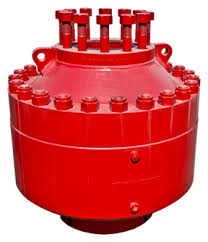
\includegraphics[scale=0.4]{images/bopannular}
\centering
\caption{A Picture of Annular BOP}
\end{figure}

\item \textbf{Ram Type Preventers:}

Ram type preventers derive their name from the twin ram elements which make up their closing mechanism. 
Three types of ram preventers are available: Blind rams - which completely close off the wellbore when 
there is no pipe in the hole.

\vspace{1em}

\end{itemize}

\begin{itemize}

\item Pipe rams - which seal off around a specific size of pipe thus
sealing of the annulus. In 1980 variable rams were made
available by manufacturers. These rams will close and seal on a
range of drill pipe sizes.


\item Shear rams which are the same as blind rams except that they
can cut through drill pipe for emergency shut-in but should only
be used as a last resort. A set of pipe rams may be installed
below the shear rams to support the severed drill string. Fig 6.2 shows the image of Pipe Ram and shear Ram BOP.

\end{itemize}


\begin{figure}[h]
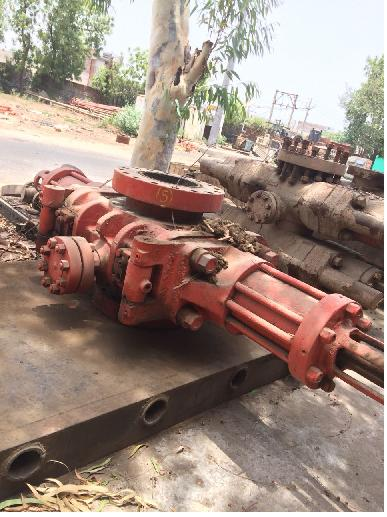
\includegraphics[scale=0.5]{images/shear_ram_BOP}
\centering 
\caption{A Picture of Pipe Ram and Shear Ram BOP}
\end{figure}

\vspace{2em}

An accumulator or Koomey unit is a unit used to hydraulically operate Rams BOP, Annular BOP, 
HCR and some hydraulic equipment. There are several of high pressure cylinders that store gas 
(in bladders) and hydraulic fluid or water under pressure for hydraulic activated systems. 
The primary purpose of this unit is to supply hydraulic power to the BOP stack in order to 
close/open BOP stack for both normal operational and emergency situation. 




